%%% Thesis Introduction --------------------------------------------------
\chapter{INTRODUCTION}
\label{chap:intro}

\graphicspath{{Introduction/IntroductionFigs/EPS/}{Introduction/IntroductionFigs/}}
\nomenclature[z1]{\cms}{Character Motion Synthesis}
\nomenclature[z2]{\cpg}{Central Pattern Generator}
\nomenclature[z3]{\dof}{Degree of Freedom}
\nomenclature[z2]{{\moit}}{Motor Invariant Theory}

\section{The Challenge}
Character Motion Synthesis (\cms) research aims at generating motion for virtual characters.
It is a topic of significant value in terms of theory and application. 
Besides major applications in the media industry, where both computer games and animation films depend heavily upon character motion for storytelling, 
current research also has applications in user interface design, psychology, sport and medicine.

The challenge of \cms  is not to make characters move, but  to make them lifelike. 
Underlying this challenge is the marvellous human ability of motion perception. 
In real life, people's motion is very similar, yet individuals vary considerably.
From the varieties in motion details, humans can infer mental states, health conditions or the surrounding environment.
%\note{uncanny valley}
Human motion perception has some very peculiar properties.
When watching a film with computer generated characters, some awkward artefacts are spotted instantly even though they are physically feasible, while many physically impossible motions are accepted as realistic and entertaining. 

%nautral looking

Nowadays in industry, high quality motions are mainly generated manually. 
Very often, characters are complex and contain a large number of joints, making animation tedious work.
To make it worse, reusing motion animation is also difficult and prone to artefacts.
Therefore high level animation tools are badly needed. 

%\note{Do An introduction for physicall based animaiton?}


Real life motions interact extensively with the environment.
Currently, the most important research endeavour is the physics based approach.
Besides  the addition of the dynamic interactive responses, it is  expected that the elimination of  artefacts that violates physics  will make motions more natural looking.
However, this paradigm faces many difficulties:
dynamics of biological systems are much more complex than artificial systems;  attempts to dynamically simulate biological system face prohibitive  computational costs and modelling difficulties.
In fact, such problems have already been identified by biological researchers.







Motor Control and Motion Perception are close related.
Difficulties in \cms reflect the inferiority of artificial control method.
The peculiarity of motion perception and control suggests  biological systems may adopt a very different principle.
To keep motions natural looking, it is worthwhile to synthesize motion following the biological motor control principle. 
This thesis is founded on new ideas from biological research.

 

\section{Agile Animals}
%\note{Underlying these problems} is our misunderstanding of animal motions.
Although animals have fascinated us for thousands of years, we still do not fully understand how they move.
Animals are very different from artificial machines and such comparisons may reflect the  biological motor control principle.
%some basic questions of motor control and motion perception remain open. 
%And answers to such questions become even more valuable nowadays. 
%Advance in this topic will greatly influence the biology, robotic engineering even intelligent research.
%\note{The difference between biological motor system}

%The paradoxes is even human are good at motor control and motion perception; human still don’t have an idea of how we move and how we perceive motion.
%Before going into details into the research ideas, we first review some puzzles troubles the foundation of CMS. 
\begin{itemize}
\HiItem {Degrees of freedom ({\dof}s)}.
From a mechanical perspective, animals have many more {\dof}s than their artificial counterparts.
An artificial ship can be approximated by a simple rigid body; whereas the flexible verteb of a fish is made up of tens of {\dof}s.


In principle, the extra {\dof}s allows for more variations in adapting the environment. 
However, for the control system, too many extra {\dof}s become a disaster because of the computational burden. 
For a human to take one step,  the neural system controls more than $600$ muscles.
Even with nowadays computer, solving this dynamics directly would spend thousands of hours.

 
\HiItem {Versatility}
Most artificial machines are designed with a single purpose, while animals are capable  of unlimited tasks.
Many biological functions which are often neglected by \cms research, such as feeding, breeding, language and vision, depend on motor control. 
Besides walking, swimming and many other styles of locomotion, we utilize many tools, such as cars, skates, bicycles and tennis rackets.

Following traditional control methods, it seems that unlimited resources need to be  allocated for motor control, while biological research shows motor control requires very few mental resources.

\HiItem{Performance}
Although the problem of biological motor control is more complex, the resulting performance surpasses artificial machines in many aspects.
Natural motions are more
\begin{enumerate} 

\HiItem{Robust:}
A human can maintain walking stability on rough terrains which would be inaccessible for vehicles.

\HiItem{Manoeuvrability and speed:}
Typical modern aeroplanes  travel at a maximum of $32\: body\: length/sec$ and yaw at $720\: deg/sec$.
While pigeons may travel at $75 \:body\: length / sec$, yaw at about  $5000 \: deg/sec$.

\HiItem{Energy Efficiency:}
The energy consumed by a walking human  is only $5\%$ of that for the world famous humanoid ASIMO.
\end{enumerate}

\end{itemize}



%For computer animation research, the key principle is we should know the things we animate.
%Natural motion system has many valuable properties which are not captured by current motion synthesis methods.
%\begin{itemize} 
% \HiItem{robust}
%Natural motions are adaptive to the changes in the environment or body conditions. 
%A common example is human locomotion. 
%Walking on different terrains will exhibit different gait while the balance is maintained. 
%
%\HiItem{speedy}
%Some motions of animals are very fast, honey birds may vibrate their wings in kHz.
%The astonishment is to the speed of motion, more puzzling is that the neural system can solve the complex motion control problem in such a short time. 
%When an animal avoids obstacles at very high running speed, 
%it must continue its running, make a turning and keep balance at the same time. 
%It seems easy for the neural system to plan complicate motions.
%\HiItem{Energy Efficient}
%Natural Motions are energy efficient.
%In theory, this idea is supported by Darwin's Theory of Evolution.
%But animals spent far less energy than our expectation.
%An example is that the energy consumed by human walking is only 5\% of that for a robot of the same scale.
%\end{itemize}

\section{Motor Invariant Theory}
\subsection{Utilizing Natural Dynamics}
Biological Motor Control has achieved a delicate balance of robustness, controllability and energy efficiency.
The real-time performance may further suggest that the biological method  is simple and requires little computational load.
These are the dreaming properties for \cms research and  the explanation that how biological systems achieve this  forms the genesis of this thesis.



At first, interactions between the body and environment pose  complex dynamic problems for motor control.
In most \cms research studies, effects of natural dynamics are treated  perturbations for planning, and are cancelled by control effort.
However from an evolutionary perspective, the mechanical structures are a product of natural selection, which has evolved alongside with the environment for millions of years. 
These structures are an advantage rather than a handicap. 
Without the need to consider stability, energy efficiency and real-time constraints,   motion can be synthesized by natural dynamics without any control effort.
Thus a new idea is that motor control is based on natural dynamics.
The neural system plays a minor role in planning; it simply utilizes natural dynamic properties.
From this perspective, the key question to be answered by Motor Invariant Theory ({\moit}) is how to utilize the natural dynamics in a systematic manner.








\subsection{Motor Invariant Theory}
%In this thesis, we propose different idea towards motor control and motion synthesis.
%In this research, we propose a different motion synthesis method based on a different motor control theory.
%
%An insightful discovery is that motor control can be “easy”.
%For some situation, some tasks mainly explore the properties of the body and environment and can be achieved with little control effort.
%In nature, we don’t finish difficult motion tasks, we select many easy motion tasks that we are good at, connect or modify them for our special purpose.
%
%The “easy” tasks are called motion primitives; they are the basic elements of our motor ability. 
%When we modify the motion primitives, some valuable properties of motion primitives are kept unchanged, and the maintained properties are called motor invariants.
%
%The inspiration of our idea comes from related biological research, which covers biomechanics and neural science.





This thesis proposes a new idea for the underlying reason for superiority of biological motor control.
It seems  that in the process of motion adaptation, some valuable properties of natural dynamics are kept invariant.
The conjecture is that:  instead of the detection and cancellation all kinds of perturbations, biological systems rely the success of motor control on  certain invariant properties of natural dynamics. 
This is \emph{Motor Invariant Theory({\moit})}.


{\moit}\ incorporates the motion primitive conjecture.
In dynamics, invariant properties are stable properties.
From a dynamic perspective, not all the motions generated by natural dynamics are stable, only a few are stable, which can be utilized as templates and become motion primitives.
The following question is how the motor control system utilizes these templates to synthesize new motion.

{\moit}\ proposes that when facing a new situation, humans do not solve motor control problems from the ground up.
Instead, our control system utilizes successful experience in similar situations.
In dynamics, adapted motions are qualitatively the same with the motion primitives or templates, and there is a one-one mapping relationship between the adapted motion and the motion primitive.
This similarity in dynamics is called topological conjugacy. 

In dynamic \cms research, a motion is represented by  a curve  $x(t)$ parameterized by $t$.
$x(t)$ is the solution to the equation (Equation ~\ref{eq:BodyEnvDym}) that describes the dynamics between the body and environment.
\begin{equation}
\dot{x}=F(x)
\label{eq:BodyEnvDym}
\end{equation}


To illustrate adaptation, we define a transformation $T$ that acts on the space of $x$.
\[
\tilde{x}=T(x)
\]

In this way, each equation can be described in two coordinate systems: one by $x$ and one by $\tilde{x}$.
As an example, Equation ~\ref{eq:EQtransform} describes the same dynamics as  Equation ~\ref{eq:tranformedEQ}.
Thus for each motion, we can obtain two equations of the transformed state~($\tilde{x}$ ) and original state $x$~(Equation ~\ref{eq:EQtransform}).

\begin{equation}
\dot{\tilde{x}}=F(\tilde{x})
\label{eq:tranformedEQ}
\end{equation}

\begin{equation}
\dot{x}=\tilde{F}(x)
\label{eq:EQtransform}
\end{equation}

Since such two equations describe the same motion, the solution of one equation can be achieved by transforming the solution of the other.
Supposing $x'(t)$ is the solution to Equation~\ref{eq:EQtransform} and $\tilde{x}(t)$ is the solution to the Equation~\ref{eq:tranformedEQ}, then we have
\[
x'(t)=T^{-1}(\tilde{x}(t))
\]
Equation~\ref{eq:tranformedEQ} and Equation~\ref{eq:BodyEnvDym} are the same, thus: 
\[
\tilde{x}(t)=x(t)
\]
Then we have
\[
x'(t)=T^{-1}(x(t))
\]

By transformation, we obtained a new motion $x'(t)$ from $x(t)$.





%if we substitue x=f(x,t) into (1).
%we can express equation (2) interm of (x,t,x)
%\dot(x)=F'(x).
%then the solution of the equation becomes 
%x2(t)=(x)t=f-1(xt)
%
%
The  transformation method has many advantages: it is much less computationally expensive and leaves many important properties untouched.
For example, if the original system ~$F$ is stable, then the transformed system $\tilde{F}$ should also be stable. 
%
In mathematical language, if there exists a continuous one-one mapping between the two dynamic systems, then the two are \emph{topological conjugate}.
This relationship is presented by $F \simeq \tilde{F}$.
$F$ and $\tilde{F}$ are called \emph{analogous systems}, which share the same topological structure.
The existence of one-one mapping is a necessary and sufficient condition for sharing topological structure.
Based on this, two  approaches for motion adaptation are developed.
Transformation can be specified explicitly or implicitly by maintaining the topology.



If the perturbation does not violate the topology, the corresponding one-one mapping will modify the motion without changing it qualitatively.
In dynamics, the topology preserving ability is an intrinsic property of many dynamic systems:
\emph{structural stability}.

One strategy of motor control is to enhance the structural stability. 
By this approach, when the qualitative property is preserved by the control system, the one-one mapping that transforms motions is automatically specified. 
However, in many cases, working out the details of one-one mapping maybe be difficult or computationally expensive.
Therefore this approach is qualitative.

In {\moit}, this approach models involuntary motion adaptations which are low level functions of the neural control system.
The topological structure is one important property that should be kept invariant, and it becomes a motor invariant in {\moit}: the \emph{Global Motor Invariant}.






Also if the transformation is known, then the two systems must be topologically equivalent.
Therefore, another approach is to directly specify the transformation.
This method  modifies motion with precision and {\moit}\ applies it to high level voluntary motor control.
In many situations, to achieve a desired transformation $T$, control effort needs to be applied.
When applying this method, how to select a proper transformation $T$ is the most challenging  question.

In {\moit}, the selection of $T$ is based on two principles.
\begin{itemize}
\item
Parameters of transformation $T$ should be easy to detect and formulate.
\item 
The transformation $T$ should be energy efficient.
For a differential dynamic system, some transformation explores the natural dynamics and requires little or no energy input.
\end{itemize}

When specifying transformation directly, some quantitative properties will be unchanged during transformation, they are \emph{Local Motor Invariant}






%the stability of the orignal system is known.
%if possible, we always try to tranform the stable motion.
%To this end motor control are applied to execute the transformation
%
%
%
%these two ideas have pros and cons.
%The first method maintail the qualitative properties, but details of motion can not be controlled precisely.
%if the second method is applied, given the transformation, the resulting motion can be know, while but to carried out such transformation, controll effort may needed.
%
%




Although the new mathematical language seems obscure at first glance, the properties that it describes are universal in physical world, with or without life.
The underlying idea is intuitive and can be explained well through commonly observed phenomena.



\subsection{The Floating Ship: An Example of Stability}
The floating ship  example shows the idea of structural stability and topological conjugacy.
In real life, typical ships have bigger height than width, as shown in Figure~\ref{fig:ShipFloating}.
An interesting  question is when floating on  waves, how the ship maintains its configuration or ``posture''.

Through analysing the topology and structural stability, we see that it requires little effort to maintain this posture.
This conclusion applies to different ships since their dynamics are qualitatively the same, or topologically conjugate.


\subsubsection*{Dynamics}

\begin{figure}[!htbp]
  \begin{center}
    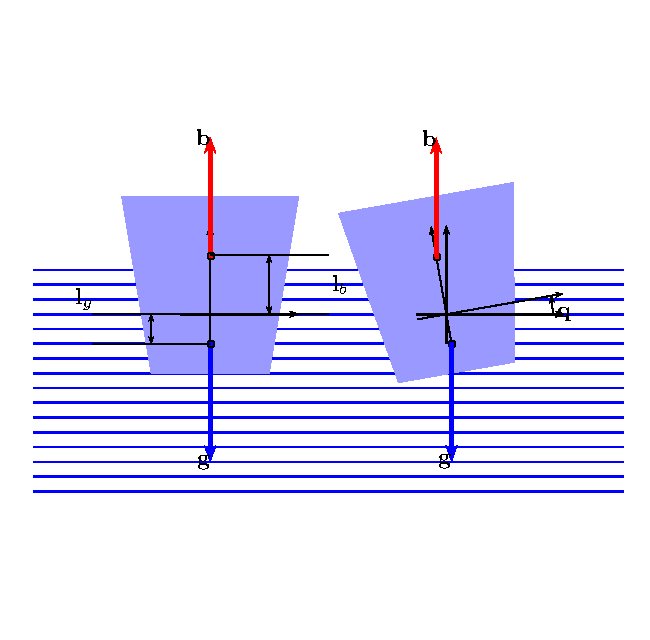
\includegraphics{ShipExample}
    \caption{The Floating Ship Example}
    \label{fig:ShipFloating}
  \end{center}
\end{figure}

The sway motion of the ship shown in Figure ~\ref{fig:ShipFloating} can be described by Equation~\ref{eq:shipflow}
\begin{equation}
\label{eq:shipflow}
J\ddot{q}+d\dot{q}=\tau(q)_{g}+\tau(q)_{b}+\tau_{u}
\end{equation}


where $q$ is the swaying angle,
$J$ is the inertia,  
$d$ is the damping coefficient,
and $\tau_{g}$,$\tau_{b}$,$\tau_{u}$ are the corresponding torques of gravity, buoyancy and external control.

When a ship is at sea, its motion is mainly governed by the two forces,  buoyancy $b$ and gravity $g$.
If $\tau_{u}=0$,  the ship motion is totally governed by the natural dynamic forces.
Such a system is \emph{autonomous}.

To make it consistent with the discussions in the following chapters, Equation~\ref{eq:shipflow} is reformulated.
By defining the \emph{state} variable $\state=[q,\qd]$,  Equation~\ref{eq:shipflow} becomes
\[
\dot{\state}=F_{J,d}(\state)+Du
\]

where 
$F$ is a function of $\state$, the subscripts~$J$ and~$d$ are \emph{system parameters},
$D$ is a matrix, which describes how the control effort is applied,
and $u$ is \emph{control input}.
For this example $u$ is $\tau_{u}$, which is $0$.



\subsubsection*{Equilibrium Postures}
A ship will only rest at the postures where $\tau_{g}+\tau_{b}+\tau_{u}=0$, which are called \emph{Equilibrium} Postures.
The only two possible ones are shown in Figure ~\ref{fig:ShipEqulibriumStable} and Figure~\ref{fig:ShipEqulibriumUnstable}.
\begin{figure}[!htbp]
  \begin{center}
     \includegraphics{leftPos}
    \caption{The Stable Equilibrium Posture}
    \label{fig:ShipEqulibriumStable}
  \end{center}
\end{figure}

\begin{figure}[!htbp]
  \begin{center}
     \includegraphics{rightPos}
    \caption{The Unstable Equilibrium Posture}
    \label{fig:ShipEqulibriumUnstable}
  \end{center}
\end{figure}



However, the two postures are different, which is illustrated with the \emph{phase plot}.
On the phase plot, the horizontal axis represents  $q$; and the vertical axis represents velocity $\qd$. 
On the phase plot, the motion of the ship is shown as a curve, which is called \emph{flow}.

The posture in Figure ~\ref{fig:ShipEqulibriumStable} is \emph{attractive} or \emph{stable}.
If a small perturbation moves the ship away from the left posture, it will return to the equilibrium posture automatically as shown in Figure~\ref{fig:StablePosture}.
\begin{figure}[!htbp]
  \begin{center}
      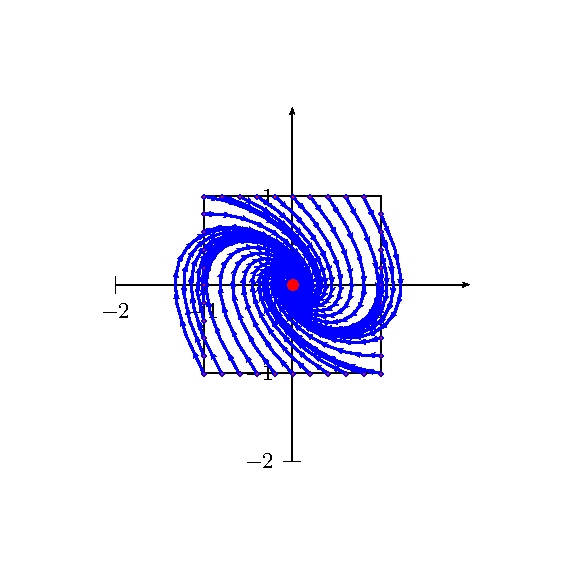
\includegraphics{stablePosition}
    \caption{Phase Plot of the Stable Posture}
    \label{fig:StablePosture}
  \end{center}
\end{figure}


Whereas the  posture in Figure~\ref{fig:ShipEqulibriumUnstable} is \emph{repelling} or \emph{unstable}, if the ship is moved away from the equilibrium posture,  by natural dynamics, it will move away even further, as shown in Figure~\ref{fig:unStablePosture}.

\begin{figure}[!htbp]
  \begin{center}
      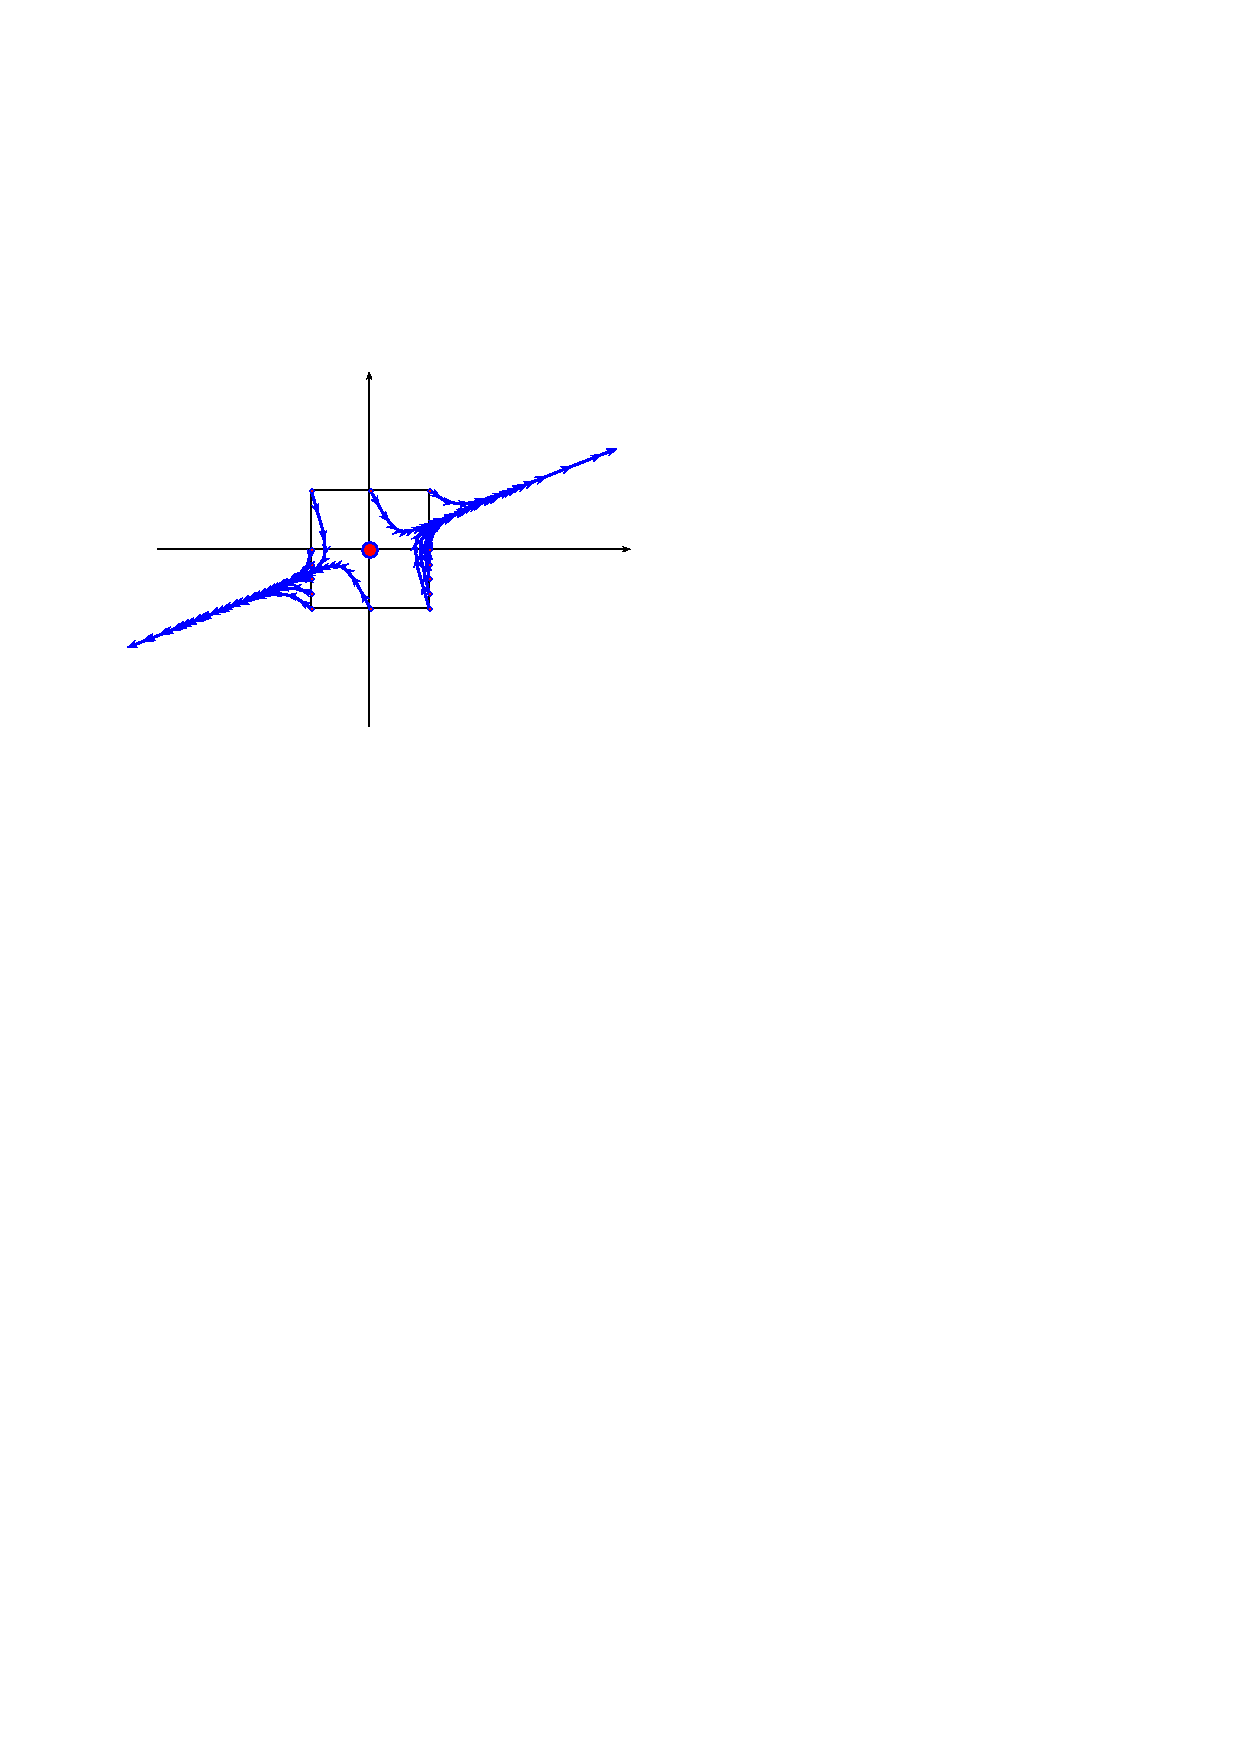
\includegraphics{unstablePosition}
    \caption{Phase Plot of the Unstable Posture}
    \label{fig:unStablePosture}
  \end{center}
\end{figure}


\subsubsection*{A Simple Task}
All the flows form the \emph{phase portrait} of the dynamic system, which illustrates all the possible motions. 
The discovery is that all the flows start from the repelling posture and end at the attractive posture.
Several curves are shown in Figure ~\ref{fig:globalflow}.
This means that no matter what the current posture, the ship will return to the normal stable posture automatically.

This is an intrinsic property of natural dynamics, and thanks to this, balancing is a simple task which requires no control effort. 
This property is determined by the qualitative structure design criterion which demands the centre of buoyancy  is above the centre of gravity.

\begin{figure}[!htbp]
  \begin{center}
   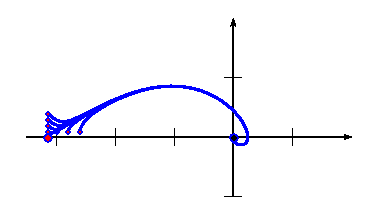
\includegraphics[width=0.7\textwidth]{ShipGlobalFlow}
   \caption{Global Properties of the Flows: All the curves start from the repelling posture~(Red) and end at the attractive one(Blue)}
   \label{fig:globalflow}
  \end{center}
\end{figure}

 



\subsubsection*{Generalization of the Ship Example} 
This conclusion is independent of the shape, size, weight or material of the ship. 
In general cases, the same wave perturbation will result in different sway motions for different ships.
However, as long as the qualitative structure design criterion is maintained, balancing remains ``easy''.
The phase portraits of all  ships share following properties. 
\begin{itemize}
\item one repelling point 
\item one attractive point 
\item all flows start from repelling point and end at the  attractive point. 
\end{itemize}

In mathematical terms, all the phase portraits share the same topological structure of Figure~\ref{fig:topologyStructure}.

This phenomenon illustrates the principal idea of motion adaptation in {\moit}.
When the variations among individuals or situations result in motion variations, the qualitative dynamics or topological structure of the dynamic system remains invariant.

\begin{figure}[!htbp]
  \begin{center}
   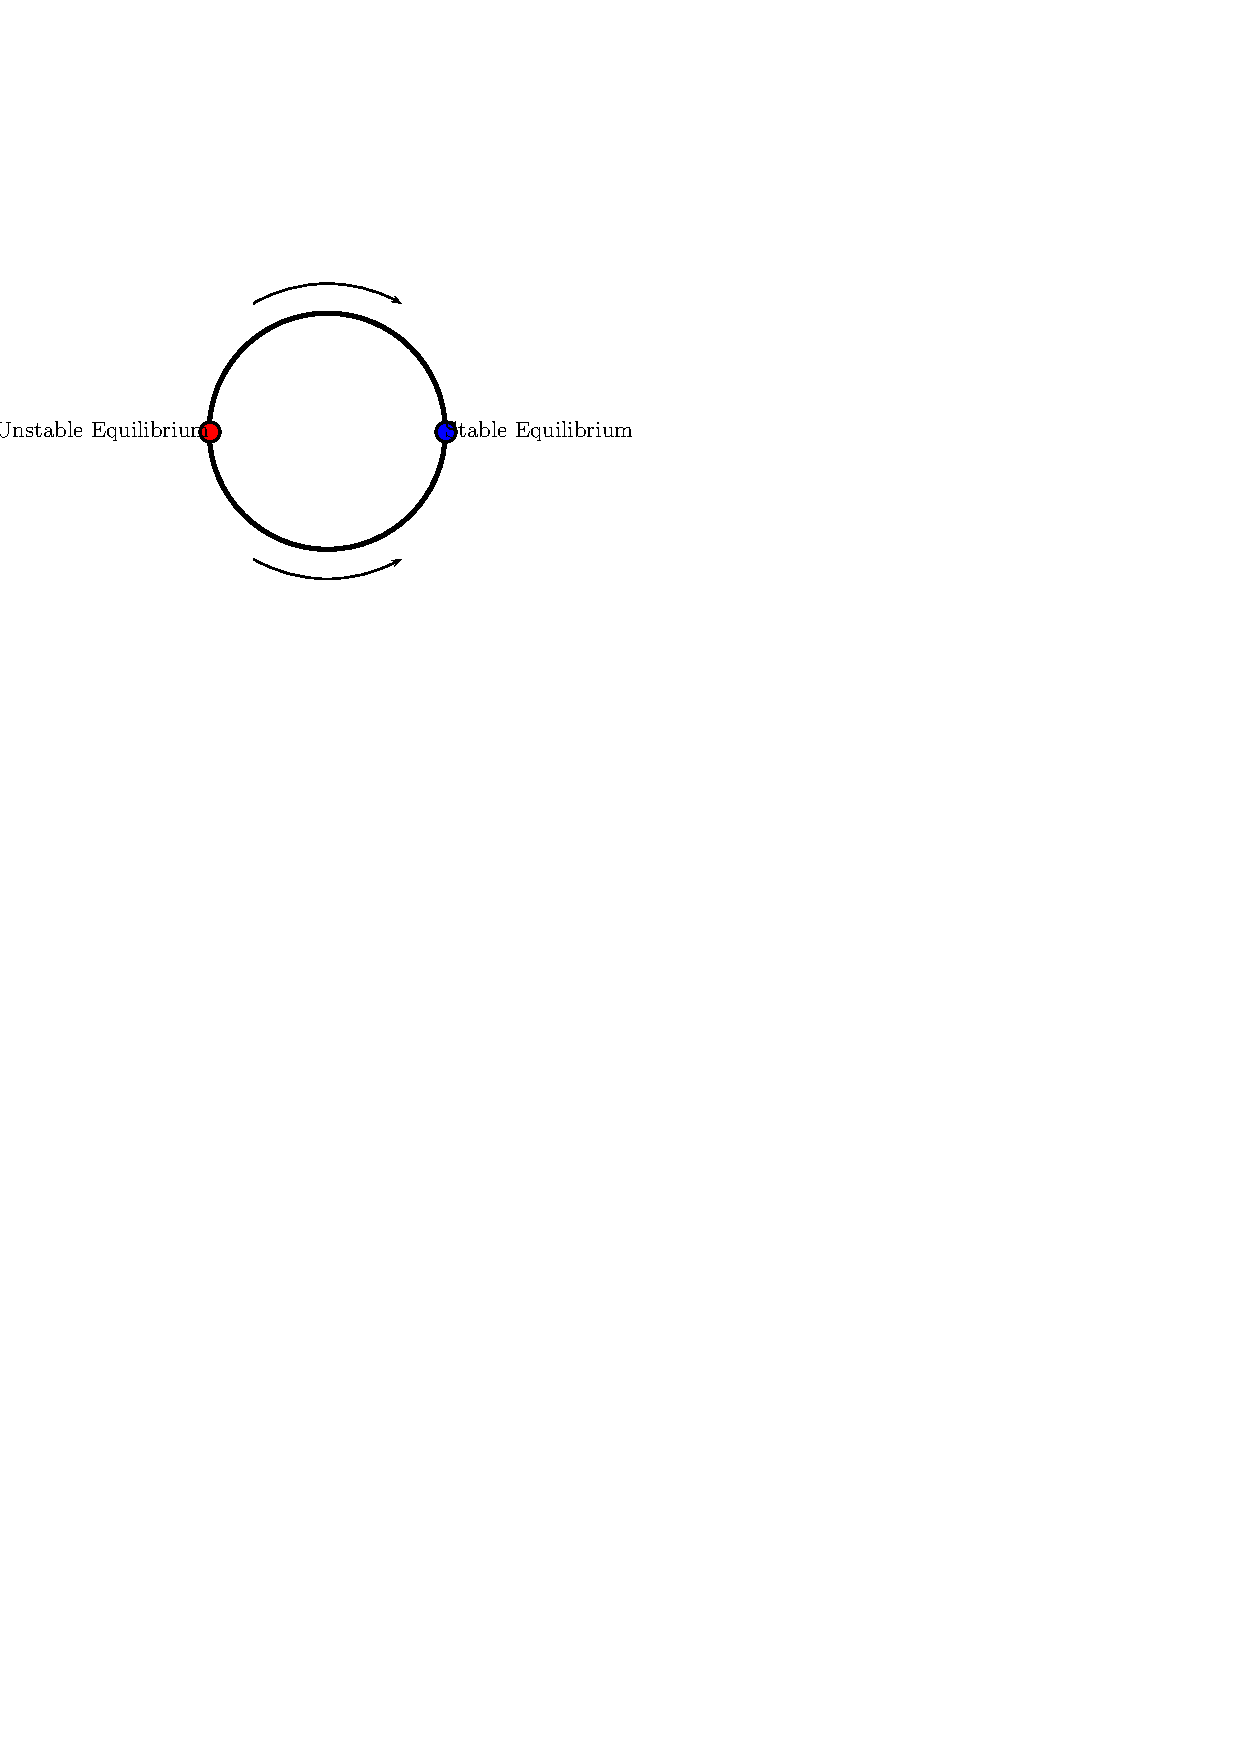
\includegraphics{topologyStructure}
   \caption{the topology  the phase portraits of ship dynamic}
   \label{fig:topologyStructure}
  \end{center}
\end{figure}




\subsection{The Mass Spring System:  Symmetry Transformation}
Despite the complexity of the body structure, biological motor control is fast and accurate.
Such quantitative properties pose another puzzle in motor control research, as solving the complex dynamics directly would require prohibitively long computational time and excessive mental resources.

{\moit}\ proposes a new method to achieve speed and accuracy in motor control.
This efficient strategy is based on the ideas of transformation and symmetry.
New motions are achieved through transforming template motions,without solving the dynamics. 
To keep the motion natural looking, the control system chooses the transformation directions that are energy efficient, or using an alternative, allowed by the natural dynamics.


Such ideas can be illustrated by the following mass spring example, shown in Figure~\ref{fig:massspring}.
The mass spring system is selected because it captures some important properties of biological dynamics.
The compliant actuators of muscles work like springs, and rigid bones are modelled as mass.


\begin{figure}[!htbp]
  \begin{center}
    \includegraphics[width=0.7\textwidth]{MassSpring}
    \caption{the mass spring system}
    \label{fig:massspring}
  \end{center}
\end{figure}

\subsubsection*{Dynamics}
The canonical equation of a mass spring system is Equation~\ref{eq:mass-spring}
\begin{equation}
\label{eq:mass-spring}
\ddot{q}+q=0.
\end{equation}
where $q$ is the offset distance.

By defining the \emph{state variable}, $\state=[q,\qd]$, Equation~\ref{eq:mass-spring} can also be reformulated in the form as
\[
\dot{\state}=F(\state)
\]

Figure~\ref{fig:massSpringPhasePlot} shows two flows passing through different states $x$ and $x'$ on the phase plot.


\begin{figure}[!htbp]
  \begin{center}
     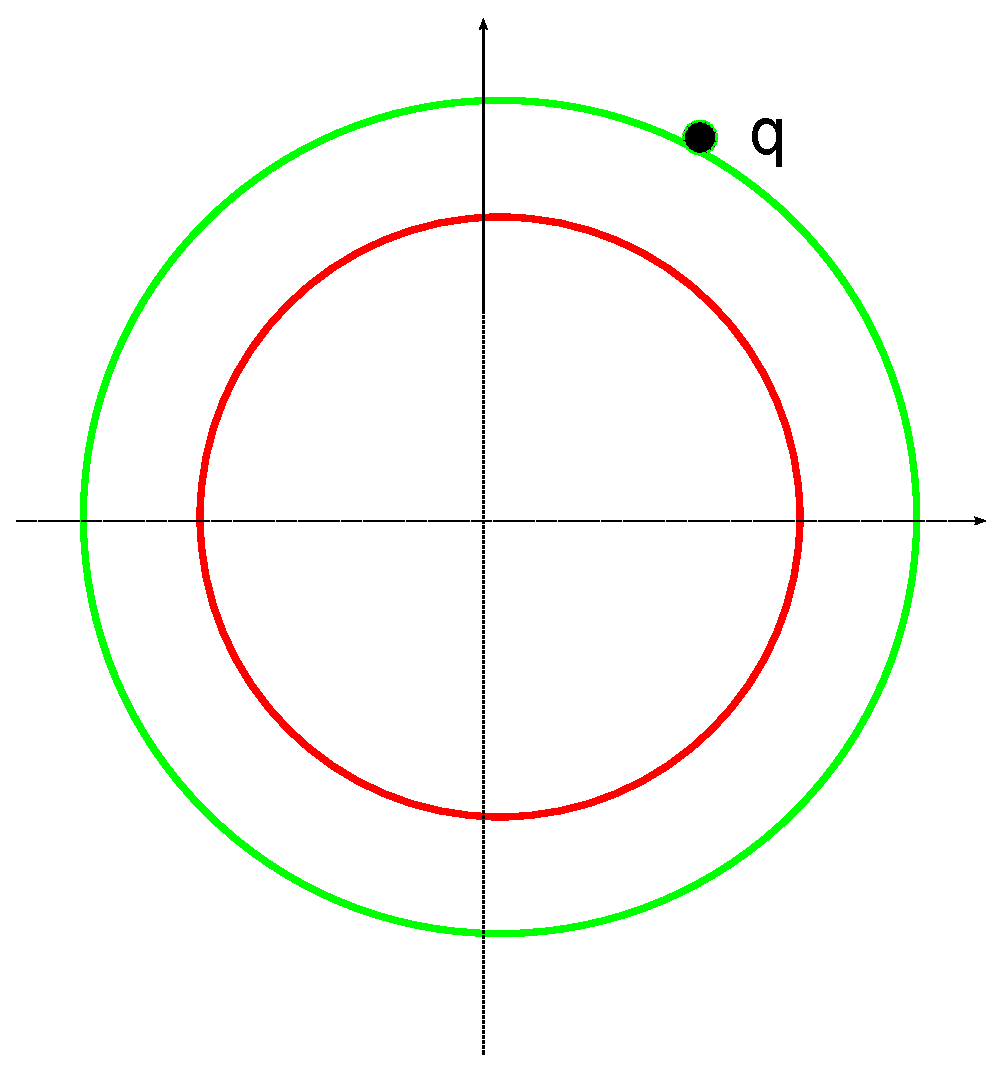
\includegraphics[width=0.5\textwidth]{MassSpringPhasePlot}
    \caption{Mass Spring Phase Plot: two flows pass through different states ($\state$ and ${\state}'$)}
    \label{fig:massSpringPhasePlot}  
  \end{center}
\end{figure}

\subsubsection*{Symmetry and Transformation}
%It is highly unlikely animals can solve Equation~\ref{eq:mass-spring}.

The mass spring system has some ``symmetrical properties''.
To an intuitive eye, different flows share the same circle ``Shape''.
Without solving the Equation~\ref{eq:mass-spring}, new flows~(solid ones) can be obtained by scaling the original~(red) flow.

From a mechanical viewpoint, this is because the flows of a mass spring system preserve energy.
To see this, we can define the energy function
\[
E=\frac{1}{2}(m\qd^2+kq^2)
\]
where $k$ is the stiffness, $m$ is the mass.
Since $E$ is a constant, we make $E=c$,
When $m=1,k=1$, we obtain
\[
 q^2+\qd^2=2c
\]
 
The equation above is the implicit function of a circle.

Therefore, given a template flow that passes through  $\state$, the flow passes through $\state'$  can be obtained by enlarge the original template flow.
In this manner, we determine the future motion after $\state'$, without solving the dynamics.


\subsubsection*{Dynamic Perception and Local Motor Invariant}

The idea of ``transformation and symmetry'' may shed light on the dynamic perception problem. 
It is highly unlikely that animals solve Equation~\ref{eq:mass-spring} to understand the the mass spring system.
As an alternative, the dynamics can be encoded in a different manner: a motion template and the symmetry property. 
If so, observed motions can be validated by checking them against our memorized motion templates.

To make it better, it is even unnecessary to work out the transformation.
In fact, it is enough just to check some property invariant under transformation.
For the example of mass spring system , we can check the ``shape'' of the flow.
For a mechanical perspective, this means to check the energy preserving property.

 
The invariant properties like preserving energy or shape can be quantitatively measured.
Since they are invariant only when flows move in a specific direction, they are called  \emph{Local Motor Invariant}. 


\subsection{Rimless Wheel}
The third example is a mechanical system with a more complex structure, the rimless wheel.
The complexity of the mechanical structure provides an opportunity to test various control ideas and compare them.

\subsubsection*{Dynamics}
The Simple 2D model is shown in Figure ~\ref{fig:rimlesswheel}. 
\begin{figure}[!htbp]
  \begin{center}
     \includegraphics[width=0.5\textwidth]{RimlessWheel}
    \caption{The Rimless Wheel}
    \label{fig:rimlesswheel}  
  \end{center}
\end{figure}
Where $\alpha$ is the angle between the spokes,  $\gamma$ is the angle of the slope,
$L$ is the length of the spoke,$\gv$ is gravity.

The dynamics of the system includes two phases: the rolling phase and the striking phase.

During the rolling phase, the rimless wheel works like a pendulum, the dynamics is as follows:
\[
\ddot{\theta}=\frac{\gv}{L}\sin(\theta+\gamma)
\]
When another spoke hits the ground, a strike happens. The impulse equation is
\[
\dot{\theta}=\cos(\alpha)\dot{\theta}
\] 

Comparing with the mass spring system, the motion of a rimless wheel is more complex. 
Depending on the initial condition, rimless wheel can roll uphill, roll downhill, stand with one spoke or stand with two spokes.
As the rimless wheel continues its motion, the final results of motion may be of any the following:
\begin{itemize}
\item rolling down the hill at a constant speed.
\item rolling down the hill at ever increasing speed.
\item stopping with one spoke as support.
\item stopping with two spokes as support.
\end{itemize}
The first one is of much interest.
In dynamics, constant rolling speed means the flow forms a limit cycle.
Figure~\ref{fig:lcofrimlesswheel} shows the limit cycle on a phase plot.
\begin{figure}[!htbp]
  \begin{center}
     \includegraphics[width=0.5\textwidth]{limitcycle}
    \caption{The Limit Cycle of The Rimless Wheel}
    \label{fig:lcofrimlesswheel}  
  \end{center}
\end{figure}




\subsubsection*{The Qualitative Approach}
The motion of a rimless wheel can be controlled by many methods.
The first method explores the topological invariant property.
For the rimless wheel system, the angle $\alpha$ between spokes and the slope angle $\gamma$ can be changed.
By doing this, we can change the constant rolling speed of the rimless wheel.
This will result in  a series of dynamic systems autonomous to the original one.
By gradually changing the parameter, on the phase plot, the limit cycle changes its shape accordingly.
The limit cycles of different mechanical parameters are shown in Figure~\ref{fig:morphyingrimlesss}

\begin{figure}[!htbp]
  \begin{center}
     \includegraphics[width=0.5\textwidth]{parameterchange}
    \caption{Different Mechanical Parameters result in Different Rimless Wheel}
    \label{fig:morphyingrimlesss}  
  \end{center}
\end{figure}



This is the qualitative approach; motion can be adapted by changing the parameter of the mechanical system. 
This method  requires no control energy input to maintain the new motion; it is energy efficient and easy to implement. 
However, the relationship between system parameters and the deformation of the limit cycle is hard to find, which prevents applying this method for tasks that require precision. 

For example, given a state on the state space, it is difficult to make limit cycle pass through the state by changing the parameters.

\subsubsection*{The Quantitative Approach}

Another approach control the rolling speed by applying control force.
For example, we apply control $u$ to the dynamic system, then the equation becomes
\[
\ddot{\theta}=\frac{\gv}{L}\sin(\theta+\gamma)+u
\]

if we set $u = \ep\frac{\gv}{L}\sin(\theta+\gamma)$, where $\ep$ is a parameter,
Then the rolling speed of the rimless wheel will be a parameter of $u$.
Figure~\ref{fig:timescalingrimlesswheel} shows two limit cycles of different $\ep$ parameter on a phase plot.
\begin{figure}[!htbp]
  \begin{center}
     \includegraphics[width=0.5\textwidth]{timescaling}
    \caption{Different Limit Cycles with Different Control}
    \label{fig:timescalingrimlesswheel}  
  \end{center}
\end{figure}

 As shown in Figure~\ref{fig:timescalingrimlesswheel}, the limit cycle is stretched vertically.
The relationship between $\ep$ and the rolling speed is simple, making this method computationally efficient and suitable for precise tasks. To make the limit cycle pass through a state $(\theta, \dot{\theta})$, if the state of same $\theta$ on the limit cycle is $ (\theta,\dot{\theta}’)$, then we have 
\[
\ep= (\frac{\dot{\theta}}{\dot{\theta}'})^2-1
\]

The disadvantage of this method is it require energy input.
Therefore for a large deformations,this method is not energy efficient.

\subsubsection*{The Difference and Comparison}
These two methods are different but related.
Neither methods will change the dynamics qualitatively. 
The systems after parameter modification,  or the controlled systems are still able to run uphill, down hill, stop with one or two spokes and roll at a constant speed.

This demonstrates the underlying topology is not changed.
Both methods try  to transform the phase portrait. 
The different transformation require different computational or energy cost.

There is another reason for choosing the rimless wheel as a example, its dynamics resemble that of animals' locomotion behaviour.
As further development, we propose this idea for motion control of dynamic characters.






\section{Contribution}

Compared with current \cms methods, the new approach has several advantages:
\begin{enumerate}
\HiItem {More Types of Adaptation.}
Most dynamic methods only focus on generating responsive motions to dynamic perturbations.
Adaptations across different characters are treated as an independent research topic~(motion re-targeting) and are tackled with very different methods.
{\moit}\ solves the two problems with one approach.
The mathematical idea of topological conjugacy  incorporates both motion re-targeting and  perturbation responses  in a unified framework.
Thus {\moit}\ is capable of more types of adaptation.
\HiItem {Better Usability.}
For many \cms methods, each \dof ~is controlled independently.
When modifying motions, the animator has to modify each \dof, which is tedious work.

In {\moit}, adaptation is achieved by applying transformation.
Each transformation can be parameterized by one parameter. 
By specifying only one parameter for the transformation, control inputs of all {\dof}s are modified automatically, making this method easier to use.

\HiItem {No Reference Motion Needed.}
{\moit}\ relies on the dynamics of body and environment.
Motion Capture Data are not needed as reference input.
In some situations, this method can generate new motion that cannot be captured.


\HiItem {Computationally Efficient.} 
This motion synthesis approach requires little computation time and memory, therefore it suits real-time applications.
\HiItem {Dynamic Motion Transition.}
Transitional motion can also be simulated dynamically, and in this research such methods have been developed upon solid theoretical foundation.

\end{enumerate}

Because of its biological foundation,
algorithms and simulation results of {\moit}\  might shed light on biology research questions.
Some conclusions and control techniques developed in this thesis provide alternative ideas for biological motor control, and have potential theoretical value.

\begin{enumerate}
\item 
The Motion Primitive Hypothesis is an old idea in biological research, but there is no agreement on the definition and underlying reasons.
Biological research has tried to identify motion primitives by exploring neural anatomy, EMG signals or muscle activation patterns.

{\moit}\ examines motion primitives from the dynamic viewpoint.
The discovery and conclusion are more logical and complete.
Besides pointing out a motion primitive, {\moit}\ also explains why certain motions become primitive, how many primitives exist, and how they are formed.


\item Many biological research ideas like \cpg and invariant based perception are proposed empirically. 
For a complete theory, much necessary detailed information is still missing.
As a contrast, {\moit}\ is based on rigid mathematical theory, for many biological ideas, {\moit}\ provides workable mathematical machinery.

\end{enumerate}







\section{Organization of the Thesis}

This thesis is organised as follows.
 
In Chapter~\ref{chap:background}, previous research on motion synthesis and biological motor control which are the motivation and justification for {\moit} are discussed, .
 
In Chapter~\ref{chap:gi},  \emph{The Qualitative Dynamics Theory} is introduced to explain motion primitives. 
Biological based  methods for maintaining the global motor invariant are developed.

Chapter~\ref{chap:li} focuses on the idea of Local Motor Invariant and Symmetry.
Lie Group Theory is  introduced  to analyse the symmetrical properties in motion dynamics.
Symmetry Controllers are developed to provide necessary energy input for adapting motions.
 


Chapter~\ref{chap:msf} discusses the combination problems.
For a single motion primitive,  strategies are developed to preserve both the global and local motor invariant simultaneously.
Motion primitive transition is discussed.
Methods for combining motion elements into more complex motions are developed.
Finally, in oder to develop an animation system, the software architecture and work flow are discussed.

Chapter~\ref{chap:gi},~\ref{chap:li} and \ref{chap:msf} lay down the theoretical foundation of {\moit}.
The following chapter provides experimental verification.



Chapter~\ref{chap:walk} focuses on the synthesizing adaptive motions for one primitive.
Bipedal walking,  which is commonly observed but poses great challenges for current \cms research,is chosen as the example,.
Methods based on {\moit}\ successfully boost the stability and generate adaptive gaits, and further validation shows the synthesized gaits comply with natural observation. 

In Chapter~\ref{chap:stance}, motion transition is discussed. 
A new balancing motion primitive is developed. 
Adaptive transitional motions from stance to walk and walk to stance are generated dynamically.


In Chapter~\ref{chap:highdor}, motor invariant theory is extended to more complex characters.
Three strategies are developed to simplify the problem for different situations.

This thesis ends with Chapter~\ref{chap:con}. 
After discussion of new finding arising from this research, some new questions and ideas for graphics and neural science are proposed for further research.





%%% ----------------------------------------------------------------------


%%% Local Variables: 
%%% mode: latex
%%% TeX-master: "../thesis"
%%% End: 

